\documentclass{beamer}

% for themes, etc.
\mode<presentation>{ 
\usetheme{Rochester} 
}

\usepackage{cancel}
\usepackage{array}
\usepackage{graphicx}
\usepackage{tikz}
\usetikzlibrary{shapes, arrows, positioning}

\title[]{Analysis of Reactor Simulations \\ Using Surrogate Models}
\subtitle[]{Thesis Defense}
\author[]{Artem Yankov}
\institute[]{University of Michigan}
\date{December 8, 2014}

% have this if you'd like a recurring outline
\AtBeginSection[]  % "Beamer, do the following at the start of every section"
{
\begin{frame}<beamer> 
\frametitle{Outline} % make a frame titled "Outline"
\tableofcontents[currentsection]  % show TOC and highlight current section
\end{frame}
}

\begin{document}

% this prints title, author etc. info from above
\begin{frame}
\titlepage
\end{frame}

% MOTIVATION
\section{Motivation}
\begin{frame}
\frametitle{Background}

\begin{itemize}
  \item Physical phenomena is studied by conducting experiments. 
  \item Any data collected represents instances of underlying stochastic processes.  
  \item We build predictive computer models in an attempt to reproduce such observed physical phenomena.
  \item To accurately capture stochastic element of experiments, computer models should be probabilistic.  
  \item In other words, inputs to computer models have uncertainties associated with them that are propagated to any outputs of interest.
  \item Running computer simulations should be like conducting physical experiments. Computer experiments.      
\end{itemize}

\end{frame}
%%%%%%%%%%%%%%%%%%%%%%%%%%%%%%%%%%%%%%%%%%%%%%%%%%%%%%%%%%%%%%%%%%%%%%%%%%%%%%%%%%%%%%%%
\begin{frame}
\frametitle{Why Surrogates?}

\begin{itemize}
  \item We run computer simulations to meet design objectives under certain constraints. 
  \item Involves numerical optimization, calibration, and performing what-if analyses.
  \item Also, we're interested in determining which of our design variables have the greatest effects on simulation outcomes. 
  \item Thousands of simulations required to make this possible but...  
  \item Computer simulations that model real phenomenon like nuclear reactors often take $\mathcal{O}(\mbox{hours})$ or $\mathcal{O}(\mbox{days})$ to complete.
  \item Building a surrogate model for your expensive computer simulations can make everything listed above possible.   
\end{itemize}

\end{frame}
%%%%%%%%%%%%%%%%%%%%%%%%%%%%%%%%%%%%%%%%%%%%%%%%%%%%%%%%%%%%%%%%%%%%%%%%%%%%%%%%%%%%%%%%
\begin{frame}
\frametitle{What is a Surrogate Model?}

\begin{itemize}
  \item A model for the outcomes of (likely) expensive computer simulations that can be rapidly evaluated while simultaneously preserving the predictive capabilities of the original simulations.
  \item Want to intelligently choose subspace $\lbrace x_1, x_2, ..., x_N\rbrace \subset \mathbf{X}$ to sample expensive computer code to get $\lbrace y_1, y_2, ..., y_N\rbrace \subset \mathbf{Y}$.
  \item Learn fast mapping that approximates $\mathbf{X}\rightarrow\mathbf{Y}$.   
\end{itemize}

\begin{figure}
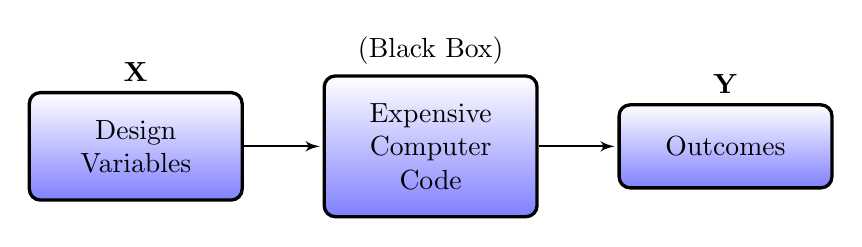
\begin{tikzpicture}[node distance=1cm, auto]  
\tikzset{
    mynode/.style={rectangle,rounded corners,draw=black, top color=white, bottom color=blue!50,very thick, inner sep=1em, minimum size=3em, text centered},
    myarrow/.style={->, >=latex', shorten >=1pt, thick},
    mylabel/.style={text width=7em, text centered} 
}  
\node[mynode, text width=2cm, label=$\mathbf{X}$] (design_vars) {Design Variables};  
\node[mynode, right= of design_vars, text width=2cm, label=(Black Box)] (computer_code) {Expensive Computer Code};
\node[mynode, right= of computer_code, text width=2cm, label=$\mathbf{Y}$] (outcomes) {Outcomes};
\draw[myarrow] (design_vars) edge node {} (computer_code);
\draw[myarrow] (computer_code) edge node {} (outcomes);
\end{tikzpicture}  
\end{figure}

\end{frame}

%%%%%%%%%%%%%%%%%%%%%%%%%%%%%%%%%%%%%%%%%%%%%%%%%%%%%%%%%%%%%%%%%%%%%%%%%%%%%%%%%%%%%%%%
\subsection{Proposed Application}
%%%%%%%%%%%%%%%%%%%%%%%%%%%%%%%%%%%%%%%%%%%%%%%%%%%%%%%%%%%%%%%%%%%%%%%%%%%%%%%%%%%%%%%%
\begin{frame}
\frametitle{Proposed Application to Fuel Performance Modeling}

\begin{itemize}
  \item Fission Gas Release (FGR) refers to the phenomenon where Xenon and Krypton gases formed in UO$_2$ fuel rods are released into the rod free volume.
  \item Causes pressure build-up and thermal conductivity degradation in the rod filling gas, potentially jeopardizing the safety of the reactor.
  \item Fission gas atoms generated in the fuel grains diffuse towards the grain boundaries. 
  \item Majority of the gas diffuses into grain-face gas bubbles, giving rise to grain-face swelling.
  \item Bubble growth brings about bubble coalescence and interconnection, eventually leading to the formation of a tunnel network through which the fission gas is released.       
\end{itemize}

\end{frame}   
%%%%%%%%%%%%%%%%%%%%%%%%%%%%%%%%%%%%%%%%%%%%%%%%%%%%%%%%%%%%%%%%%%%%%%%%%%%%%%%%%%%%%%%%
\begin{frame}
\frametitle{Bison: Fuel Perfromance Modeling Code}  

\begin{columns}
 \begin{column}{0.6\textwidth}

\begin{itemize}
  \item A finite-element based, parallel, fully-coupled nuclear fuel performance code under development at Idaho National Laboratory.
  \item Models complex, multiphysics phenomena occurring over distances ranging from inter-atomic spacing to meters, time scales from $\mu s$ to years. 
  \item Simulations have required as many as 12,000 CPUs. Bison is as expensive as codes get.    
\end{itemize}

 \end{column}

 \begin{column}{0.4\textwidth}
  \centering
  \includegraphics[width=1.\textwidth, totalheight=0.45\textheight]{./bison_mesh.png} \\
  \includegraphics[width=1.\textwidth, totalheight=0.45\textheight]{./bison_is_stud.png}
 \end{column}
\end{columns}

\footnotetext[1]{\tiny Richard Williamson et. al. Overview of the BISON Multidimensional Fuel Performance Code. IAEA Technical Meeting: Modeling of Water-Cooled Fuel Including Design-Basis and Severe Accidents. Oct. 28, Chengdu, China.}

\end{frame}
%%%%%%%%%%%%%%%%%%%%%%%%%%%%%%%%%%%%%%%%%%%%%%%%%%%%%%%%%%%%%%%%%%%%%%%%%%%%%%%%%%%%%%%%
\begin{frame}
\frametitle{SIFGRS FGR Model}

\begin{itemize}
  \item Simple Integrated Fission Gas Release and Swelling (SIFGRS)
  \item Incorporates gas diffusion and precipitation in grains, growth and coalescence of gas bubbles at grain faces, thermal, athermal, steady-state, and transient gas release. 
  \item Through a direct description of the grain face gas bubble development, the fission gas swelling and release are calculated as coupled processes.
  \item Parameterized by, among others, linear heat rate, gas diffusion coefficient, surface tension of grain face bubbles, hydrostatic pressure, fuel grain radius, fuel porosity, and grain boundary sweeping. 
\end{itemize}

\end{frame}
%%%%%%%%%%%%%%%%%%%%%%%%%%%%%%%%%%%%%%%%%%%%%%%%%%%%%%%%%%%%%%%%%%%%%%%%%%%%%%%%%%%%%%%%
\begin{frame}
\frametitle{Ris\o~AN3 Experiment}

\begin{itemize}
  \item Validation case for fuel performance modeling in the Fumex-II database.
  \item Experiment consists of a base irradiation of four reactor cycles in the Biblis A pressurized water reactor.
  \item After the base irradiation period, a fuel rod is extracted and refabricated to a shorter length before undergoing a power ramp.
  \item Refabricated fuel rod is outfitted with various instrumentation such that fuel centerline temperature, FGR and rod internal pressure measurements can be obtained.    
\end{itemize}

\end{frame}
%%%%%%%%%%%%%%%%%%%%%%%%%%%%%%%%%%%%%%%%%%%%%%%%%%%%%%%%%%%%%%%%%%%%%%%%%%%%%%%%%%%%%%%%
\begin{frame}
\frametitle{Ris\o~AN3 Experiment Irradiation Profiles}

\begin{columns}
 \begin{column}{0.5\textwidth}
  \centering
  Base Irradiation History
  \includegraphics[width=1.\textwidth]{./base_irrad.png}
 \end{column}
 \begin{column}{0.5\textwidth}
  \centering
  Power Ramp Experiment \\ (This is what we're modeling)
  \includegraphics[width=1.\textwidth]{./power_ramp.png}
 \end{column}
\end{columns}

\end{frame}
%%%%%%%%%%%%%%%%%%%%%%%%%%%%%%%%%%%%%%%%%%%%%%%%%%%%%%%%%%%%%%%%%%%%%%%%%%%%%%%%%%%%%%%%
\begin{frame}
\frametitle{Modeling Ris\o~AN3 Experiment with Bison}

\begin{columns}
 \begin{column}{0.7\textwidth}

\begin{itemize}
  \item Fuel rod modeled as two fuel pellets smeared together.
  \item The first pellet has a hole down the center. Mesh consists of 29 axial nodes and 10 radial nodes.
  \item Second pellet has no hole down the center. Mesh consists of 166 axial nodes and 13 radial nodes.
  \item The clad mesh consists of 131 axial nodes and 3 radial nodes. 
  \item A 2-dimensional axi-symmetric quadratic element mesh used. 
\end{itemize}

 \end{column}
 \begin{column}{0.3\textwidth}
  \centering
  Bison Mesh
  \includegraphics[width=1.\textwidth]{./riso_an3_mesh.png}
 \end{column}
\end{columns}

\end{frame}
%%%%%%%%%%%%%%%%%%%%%%%%%%%%%%%%%%%%%%%%%%%%%%%%%%%%%%%%%%%%%%%%%%%%%%%%%%%%%%%%%%%%%%%%
%\begin{frame}
%\frametitle{Modeling Ris\o~AN3 Experiment with Bison}
%
%\begin{itemize}
%  \item SIFGRS parameters are quite generic and uncertain. 
%  \item Bison over-predicts FGR by a factor of 2 some 40 hours into the power ramp.
%\end{itemize}
%
%\begin{columns}
% \begin{column}{0.5\textwidth}
%  \centering
%  Fission Gas Release
%  \includegraphics[width=1.\textwidth]{./fgr_comparison.png}
% \end{column}
% \begin{column}{0.5\textwidth}
%  \centering
%  Fuel Centerline Temperature
%  \includegraphics[width=1.\textwidth]{./tc_temp_comparison.png}
% \end{column}
%\end{columns}
%
%\end{frame}
%%%%%%%%%%%%%%%%%%%%%%%%%%%%%%%%%%%%%%%%%%%%%%%%%%%%%%%%%%%%%%%%%%%%%%%%%%%%%%%%%%%%%%%%
\begin{frame}
\frametitle{Ris\o~AN3 Experiment}

\begin{itemize}
  \item Bison does a good job predicting fuel centerline temperature, very strongly correlated to power.
\end{itemize}

\begin{columns}
 \begin{column}{0.5\textwidth}
  \centering
  Power Ramp Experiment
  \includegraphics[width=1.\textwidth]{./power_ramp.png}
 \end{column}
 \begin{column}{0.5\textwidth}
  \centering
  Fuel Centerline Temperature
  \includegraphics[width=1.\textwidth]{./tc_temp_comparison.png}
 \end{column}
\end{columns}

\end{frame}
%%%%%%%%%%%%%%%%%%%%%%%%%%%%%%%%%%%%%%%%%%%%%%%%%%%%%%%%%%%%%%%%%%%%%%%%%%%%%%%%%%%%%%%%
\begin{frame}
\frametitle{Ris\o~AN3 Experiment}

\begin{itemize}
  \item Bison over-predicts FGR by a factor of 2 some 40 hours into the power ramp.
\end{itemize}

\begin{columns}
 \begin{column}{0.5\textwidth}
  \centering
  Power Ramp Experiment
  \includegraphics[width=1.\textwidth]{./power_ramp.png}
 \end{column}
 \begin{column}{0.5\textwidth}
  \centering
  Fission Gas Release
  \includegraphics[width=1.\textwidth]{./fgr_comparison.png}
 \end{column}
\end{columns}

\end{frame}
%%%%%%%%%%%%%%%%%%%%%%%%%%%%%%%%%%%%%%%%%%%%%%%%%%%%%%%%%%%%%%%%%%%%%%%%%%%%%%%%%%%%%%%%
\begin{frame}
\frametitle{Modeling Ris\o~AN3 Experiment with Bison}

\begin{itemize}
  \item Bison predictions of FGR and temperature fields stand to be improved by calibrating FGR parameters to experimental data.
  \item Calibration studies require $\mathcal{O}(10^3)$ function evaluations, which in this research is the Bison computer code.
  \item Each simulation of the Ris\o~AN3 experiment will take a few hours on multiple processors.
  \item It's necessary to construct a surrogate for the calibration study. 
\end{itemize}

\end{frame}


% SURROGATE CONSTRUCTION
\section{Surrogate Models}
% OVERVIEW
\subsection{Overview}
%%%%%%%%%%%%%%%%%%%%%%%%%%%%%%%%%%%%%%%%%%%%%%%%%%%%%%%%%%%%%%%%%%%%%%%%%%%%%%%%%%%%%%%%
\begin{frame}
\frametitle{Classic Overview}

\begin{figure}
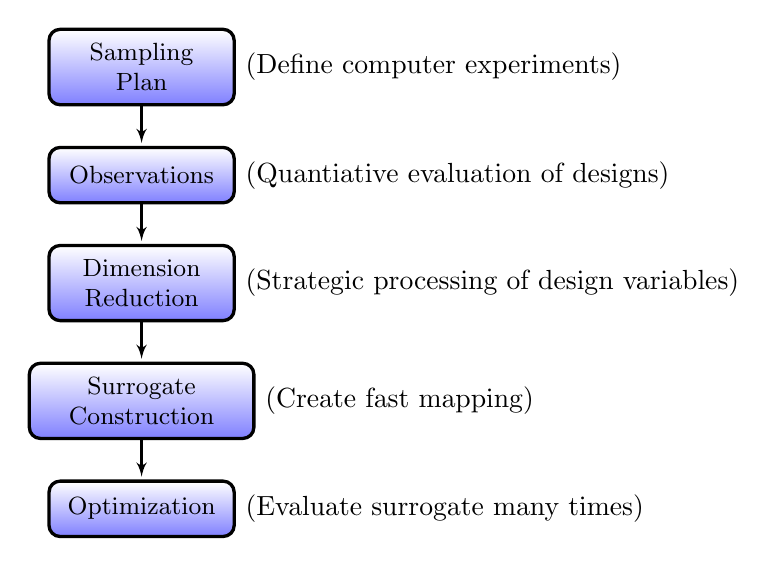
\begin{tikzpicture}[node distance=0.5cm, auto]  
\tikzset{
    mynode/.style={rectangle,rounded corners,draw=black, top color=white, bottom color=blue!50, very thick, inner sep=.5em, minimum size=2em, text centered, font=\small},
    myarrow/.style={->, >=latex', shorten >=1pt, thick}
}  
\node[mynode, text width=2cm, label=right:(Define computer experiments)](samp_plan) {Sampling Plan};
\node[mynode, below= of samp_plan, text width=2cm, label=right:(Quantiative evaluation of designs)](obs) {Observations};
\node[mynode, below= of obs, text width=2cm, label=right:(Strategic processing of design variables)](dim_red) {Dimension Reduction};
\node[mynode, below= of dim_red, text width=2.5cm, label=right:(Create fast mapping)](surr) {Surrogate Construction};
\node[mynode, below= of surr, text width=2cm, label=right:(Evaluate surrogate many times)](opt) {Optimization};
\draw[myarrow] (samp_plan) edge node {} (obs);
\draw[myarrow] (obs) edge node {} (dim_red);
\draw[myarrow] (dim_red) edge node {} (surr);
\draw[myarrow] (surr) edge node {} (opt);
\end{tikzpicture}  
\end{figure}

\end{frame}
%%%%%%%%%%%%%%%%%%%%%%%%%%%%%%%%%%%%%%%%%%%%%%%%%%%%%%%%%%%%%%%%%%%%%%%%%%%%%%%%%%%%%%%%
\begin{frame}
\frametitle{Kriging vs. anchored-ANOVA Collocation}

\begin{itemize}
  \item Kriging has been around since the 1950s while anchored-ANOVA collocation approach had been developed in the 2000s. 
  \item anchored-ANOVA collocation showed great promise in applications in other engineering fields.
  \item Both surrogate approaches were tested for their ultimate applicability to a difficult problem in fuel performance modeling.
  \item Tested on infinite lattice problem, 3-by-3 minicore in PARCS, and simple point kinetics/thermalhydraulics problem.  
  \item Received major DOE grant in Winter, 2013 to apply surrogates to fuel performance modeling. Focus area changed.
\end{itemize}

\end{frame}
%%%%%%%%%%%%%%%%%%%%%%%%%%%%%%%%%%%%%%%%%%%%%%%%%%%%%%%%%%%%%%%%%%%%%%%%%%%%%%%%%%%%%%%%
\begin{frame}
\frametitle{Kriging vs. anchored-ANOVA Collocation}

\begin{columns}
 \begin{column}{0.5\textwidth}
  Kriging
  \begin{itemize}
    \item Dimension reduction processed separately
    \item Sampling points random
    \item User determines how many points to use for sampling plan
    \item Interpolation by covariance basis functions
    \item More statistical approach
  \end{itemize}
 \end{column}
 \begin{column}{0.5\textwidth}
 anchored-ANOVA Collocation
  \begin{itemize}
    \item Dimension reduction inherent
    \item Sampling done on structured grid
    \item Sampling plan size dependent on number of design variables
    \item Polynomial interpolation
    \item More deterministic approach
  \end{itemize}
 \end{column}
\end{columns}

\end{frame}
%%%%%%%%%%%%%%%%%%%%%%%%%%%%%%%%%%%%%%%%%%%%%%%%%%%%%%%%%%%%%%%%%%%%%%%%%%%%%%%%%%%%%%%%
\begin{frame}
\frametitle{Lessons Learned in Applying Surrogate Methodologies}

\begin{itemize}
  \item Non-linearity of fission gas release models coupled with large uncertainties implied the need for modeling higher-order interaction effects. 
  \item Modeling such higher-order effects with anchored-ANOVA and Smolyak sparse grids can get very expensive, with no clear limit of how many objective function simulations will be needed. 
  \item Transparency of Kriging appealing when considering each Bison fission gas release simulation would have to be performed in parallel.
  \item If simulations fail to converge or experiences an error, the correction process is straight forward. Contrarily, there are a lot of moving pieces in the anchored-ANOVA surrogate approach. 
  \item Clear extension to time series. 
\end{itemize}

\end{frame}
%%%%%%%%%%%%%%%%%%%%%%%%%%%%%%%%%%%%%%%%%%%%%%%%%%%%%%%%%%%%%%%%%%%%%%%%%%%%%%%%%%%%%%%%
\subsection{Kriging}

%%%%%%%%%%%%%%%%%%%%%%%%%%%%%%%%%%%%%%%%%%%%%%%%%%%%%%%%%%%%%%%%%%%%%%%%%%%%%%%%%%%%%%%%
\begin{frame}
\frametitle{Dimension Reduction for Kriging}

\begin{itemize}
  \item Kriging effective for $\mathcal{O}(10)$ design variables.
  \item For more design variables Kriging will defeat the purpose of having a surrogate in the first place.
  \item Fortunately, various engineering applications have shown that only a handful of design variables have non trivial impact on outputs of interest.
  \item How to identify the "important variables"?
  \item Morris' Algorithm.   
\end{itemize}

\end{frame}
%%%%%%%%%%%%%%%%%%%%%%%%%%%%%%%%%%%%%%%%%%%%%%%%%%%%%%%%%%%%%%%%%%%%%%%%%%%%%%%%%%%%%%%%
\begin{frame}
\frametitle{Morris' Algorithm}

\begin{itemize}
  \item Premise: If the output parameter does not change with respect to a design variable then the variable can safely be ignored.
  \item Elementary effect $d_i\left(\textbf{x}\right)$ of design variable $x_i$:
\begin{align*}
 d_i\left(\textbf{x}\right) = \frac{f\left(x_1,x_2,...,x_{i-1},x_i+\Delta,x_{i+1},....,x_k 									\right) - f\left(\textbf{x}\right)}{\Delta}      
\end{align*} 
  \item Choosing a set of $\textbf{x}$ carefully, it is possible to calculate an elementary effect for each of $k$ design variables using only $k+1$ function evaluations using the random orientation matrix $\textbf{B}^*$: 
\begin{align*}
 \textbf{B}^* = \left(\textbf{1}_{k+1,1}\textbf{x}^* + \frac{\Delta}{2}\left[
                 \left(2\textbf{B} - \textbf{1}_{k+1,k}\right)\textbf{D}^* + 
                  \textbf{1}_{k+1,k}\right]\right)\textbf{P}^*.
\end{align*}                
\end{itemize}

\end{frame}
%%%%%%%%%%%%%%%%%%%%%%%%%%%%%%%%%%%%%%%%%%%%%%%%%%%%%%%%%%%%%%%%%%%%%%%%%%%%%%%%%%%%%%%%
\begin{frame}
\frametitle{Morris' Algorithm}

\begin{itemize}
  \item $r$ random orientation matrices are created to obtain $r$ elementary effects for each design variable. 
  \item Plot mean and standard deviation of each variable's effects.
  \item Variables with negligible effect on function will cluster around origin. 
  \item Large fluctuations in standard deviation indicative of nonlinear and interactive effects.              
\end{itemize}

\centering
\includegraphics[width=0.50\textwidth]{./morris_alg.png}

\end{frame}
%%%%%%%%%%%%%%%%%%%%%%%%%%%%%%%%%%%%%%%%%%%%%%%%%%%%%%%%%%%%%%%%%%%%%%%%%%%%%%%%%%%%%%%%
\begin{frame}
\frametitle{Designing a Kriging Sampling Plan}

\begin{itemize}
  \item All surrogate models are built around a set of points at which the objective computer code is actually evaluated. 
  \item Intuitively, the surrogate accuracy is expected to decrease as one moves further away from such points. 
  \item Important to spread $N$ points as uniformly as possible across the design space.
  \item For Kriging, Latin Hypercube Sampling (LHS) is used to create a sampling plan.
  \item There is a notion of an optimized LHS sampling plan based on the maximin metric.   
\end{itemize}

\end{frame}
%%%%%%%%%%%%%%%%%%%%%%%%%%%%%%%%%%%%%%%%%%%%%%%%%%%%%%%%%%%%%%%%%%%%%%%%%%%%%%%%%%%%%%%%
\begin{frame}
\frametitle{Latin Hypercube Sampling}

\begin{itemize}
  \item Basis of LHS rests upon dividing the normalized space of each design variable into $n$ equally sized bins if $n$ samples are required. 
  \item As a result, when the $n$ samples are taken it is guaranteed that the entire
spectrum of each design variable's space has been visited.  
\end{itemize}
\centering
\includegraphics[width=0.58\textwidth]{./lhs.png}

\end{frame}
%%%%%%%%%%%%%%%%%%%%%%%%%%%%%%%%%%%%%%%%%%%%%%%%%%%%%%%%%%%%%%%%%%%%%%%%%%%%%%%%%%%%%%%%
\begin{frame}
\frametitle{Optimizing a LHS Plan}

\begin{itemize}
  \item The maximin metric describe by Morris and Mitchell makes use of two notions in an attempt to quantify the 'space-fillingness' of a sampling plan. 
  \item Unique distances between all points in the plan sorted in ascending order $\lbrace d_1, d_2, ..., d_m\rbrace$.
  \item Corresponding number of occurrences of each distance $\lbrace J_1, J_2, ..., J_m\rbrace$.  
  \item In words, the Morris and Mitchell criteria states that an optimized sampling plan will minimize all $J_i$ while maximizing the corresponding $d_i$. 
  \item The maximin sampling plan maximizes $d_1$, and among plans for which this is true, minimizes $J_1$, among plans for which this is true, maximizes $d_2$,....
\end{itemize}

\end{frame}
%%%%%%%%%%%%%%%%%%%%%%%%%%%%%%%%%%%%%%%%%%%%%%%%%%%%%%%%%%%%%%%%%%%%%%%%%%%%%%%%%%%%%%%%
\begin{frame}
\frametitle{Optimizing a LHS Plan}

\begin{itemize}
  \item The previous definition can be restated into a pseudo equivalent minimization problem.
\begin{equation}
\label{eq:Phi_q}
   \Phi_q(\textbf{X}) = \left(\sum_{j=1}^m J_j d_j^{-q} \right)^{1/q} \nonumber
\end{equation}
  \item The minimization of this equation and the Morris and Mitchell definition of the maximin sampling plan are used in unison to obtain a locally optimal sampling plan.
  \item Generate initial sampling plan, optimize for set of $q$ values using simulated annealing.  
  \item Resulting set of plans are contested directly against each other by explicit application of Morris and Mitchell's maximin definition. 
\end{itemize}

\end{frame}
%%%%%%%%%%%%%%%%%%%%%%%%%%%%%%%%%%%%%%%%%%%%%%%%%%%%%%%%%%%%%%%%%%%%%%%%%%%%%%%%%%%%%%%%
\begin{frame}
\frametitle{Kriging}

\begin{itemize}
  \item Linear regression is most commonly used surrogate to model a stochastic process.

\begin{equation}
   y\left( \textbf{x}^{(i)} \right) = \sum_h \beta_h f_h\left( \textbf{x}^{(i)} \right) + \epsilon^{(i)} \nonumber
\end{equation}

  \item The $\epsilon^{(i)}$ are normally distributed, independent error terms with mean $0$ and variance $\sigma^2$.
  \item The assumption of independent error terms is wrong. Errors are correlated. 
\end{itemize}

\end{frame}
%%%%%%%%%%%%%%%%%%%%%%%%%%%%%%%%%%%%%%%%%%%%%%%%%%%%%%%%%%%%%%%%%%%%%%%%%%%%%%%%%%%%%%%%
\begin{frame}
\frametitle{Kriging}

\begin{itemize}
  \item Given that error terms should be correlated, what if we modeled the error terms instead of the mean?

\begin{equation}
   d\left( \textbf{x}^{(i)}, \textbf{x}^{(j)} \right) = \sum_{h=1}^{k} \theta_h \left| x_h^{(i)} - x_h^{(j)} \right|^{p_h} \nonumber
\end{equation}

\begin{equation}
   \text{cor} \left[ \epsilon\left( \textbf{x}^{(i)} \right) , \epsilon\left( \textbf{x}^{(j)} \right)  \right] =
      \exp\left[ -d\left( \textbf{x}^{(i)}, \textbf{x}^{(j)} \right) \right]  \nonumber
\end{equation}

  \item This is what Kriging does.

\begin{equation}
   y\left( \textbf{x}^{(i)} \right) = \mu + \epsilon\left( \textbf{x}^{(i)} \right) \nonumber
\end{equation}

\end{itemize}

\end{frame}
%%%%%%%%%%%%%%%%%%%%%%%%%%%%%%%%%%%%%%%%%%%%%%%%%%%%%%%%%%%%%%%%%%%%%%%%%%%%%%%%%%%%%%%%
\begin{frame}
\frametitle{Kriging on a Sampling Plan}

\begin{itemize}
  \item Optimized sampling plan $\textbf{X}=\lbrace \textbf{x}^{(1)}, \textbf{x}^{(2)}, ... \textbf{x}^{(n)}\rbrace$. 
  \item At each datum $\textbf{x}^{(k)}$ a random process $Y(\textbf{x}^{(i)})$ induces an observation $y^{(i)}$.
  \item Resulting random field can be described with a mean value of $\textbf{1}\mu$ and a correlation matrix,
\begin{equation}
 \boldsymbol{\Psi} =
 \begin{pmatrix} 
	\text{cor} \left[ \epsilon\left( \textbf{x}^{(1)} \right) , \epsilon\left( \textbf{x}^{(1)} \right)  \right] & \cdots & 
		\text{cor} \left[ \epsilon\left( \textbf{x}^{(1)} \right) , \epsilon\left( \textbf{x}^{(n)} \right)  \right]  \\
	\vdots & \ddots & \vdots \\ 
	\text{cor} \left[ \epsilon\left( \textbf{x}^{(n)} \right) , \epsilon\left( \textbf{x}^{(1)} \right)  \right]  & \cdots & 
		\text{cor} \left[ \epsilon\left( \textbf{x}^{(n)} \right) , \epsilon\left( \textbf{x}^{(n)} \right)  \right] 
 \end{pmatrix} \nonumber
\end{equation}  

\end{itemize}

\end{frame}
%%%%%%%%%%%%%%%%%%%%%%%%%%%%%%%%%%%%%%%%%%%%%%%%%%%%%%%%%%%%%%%%%%%%%%%%%%%%%%%%%%%%%%%%
\begin{frame}
\frametitle{Kriging on a Sampling Plan}

\begin{itemize}
  \item Given the formulation of the observations occurring at $\textbf{x}^{(k)}$ as instances of a stochastic process, the likelihood of seeing the observed data is,
\begin{eqnarray}
   L\left(\textbf{Y}^{(1)}, ..., \textbf{Y}^{(n)} | 
    \mu, \sigma, \lbrace \theta_1,..., \theta_k\rbrace, 
    \lbrace p_1,..., p_k\rbrace\right) = \nonumber \\
     \frac{1}{\left(2\pi\sigma^2\right)^{n/2}|\boldsymbol{\Psi}|^{1/2}}\times
     \exp\left[\frac{  \left(\textbf{y}-\textbf{1}\mu\right)^T
    \boldsymbol{\Psi}^{-1} \left(\textbf{y}-\textbf{1}\mu\right)}
    {2\sigma^2} \right] . \nonumber
\end{eqnarray} 
  \item Maximizing the log likelihood, 
   \begin{equation}
   	\hat{\mu} = \frac{ \textbf{1}^T\boldsymbol{\Psi}^{-1}\textbf{y} }
    		 	    {  \textbf{1}^T\boldsymbol{\Psi}^{-1}\textbf{1} } \nonumber
   \end{equation}
   \begin{equation}
   	\hat{\sigma}^2 = \frac{  \left(\textbf{y}-\textbf{1}\mu\right)^T
    			\boldsymbol{\Psi}^{-1} \left(\textbf{y}-\textbf{1}\mu\right)}{n}. \nonumber
   \end{equation}
\end{itemize}

\end{frame}
%%%%%%%%%%%%%%%%%%%%%%%%%%%%%%%%%%%%%%%%%%%%%%%%%%%%%%%%%%%%%%%%%%%%%%%%%%%%%%%%%%%%%%%%
\begin{frame}
\frametitle{Kriging on a Sampling Plan}

\begin{itemize}
  \item Substitute $\hat{\sigma}$ and $\hat{\mu}$ into log likelihood to get, concentrated ln-likelihood function.
   \begin{equation}
    \log(L) \approx -\frac{n}{2}\log\left(\hat{\sigma}^2\right) -
     \frac{1}{2} \log|\boldsymbol{\Psi}| \nonumber	
   \end{equation}
  \item Optimize with respect to the $\theta$ and $p$ parameters using global search algorithm.
  \item Once all optimizing parameters are available the goal is to utilize the parameters to build a model that makes function predictions on new points $\textbf{x}$.
\end{itemize}

\end{frame}
%%%%%%%%%%%%%%%%%%%%%%%%%%%%%%%%%%%%%%%%%%%%%%%%%%%%%%%%%%%%%%%%%%%%%%%%%%%%%%%%%%%%%%%%
\begin{frame}
\frametitle{Making Predictions with Kriging Surrogate}

\begin{itemize}
  \item Construct a vector of correlations with existing points and $\textbf{x}$,
   \begin{equation}
 	\boldsymbol{\psi} =
 	\begin{pmatrix} 
	 \text{cor} \left[ \epsilon\left( \textbf{x}^{(1)} \right) , \epsilon\left( \textbf{x} \right)  \right]  \\
	 \vdots \\ 
	 \text{cor} \left[ \epsilon\left( \textbf{x}^{(n)} \right) , \epsilon\left( \textbf{x} \right)  \right] 
    \end{pmatrix}. \nonumber
   \end{equation} 
  \item  New predictions can be made at $\textbf{x}$ using the maximum likelihood estimator,
   \begin{equation}
    \hat{y}(\textbf{x}) = \hat{\mu} + 
   	 \boldsymbol{\psi}^T\boldsymbol{\Psi}^{-1}
   	  \left(\textbf{y} - \textbf{1}\hat{\mu}\right). \nonumber
   \end{equation}
  \item Prediction using kriging works to estimate a function value at a certain point by computing a weighted average of known function values in the vicinity of the objective points.
\end{itemize}

\end{frame}

% Application to FGR
\section{Application to Fission Gas Release}
% What is FGR
\subsection{FGR Background}
%%%%%%%%%%%%%%%%%%%%%%%%%%%%%%%%%%%%%%%%%%%%%%%%%%%%%%%%%%%%%%%%%%%%%%%%%%%%%%%%%%%%%%%%
\begin{frame}
\frametitle{High Level Overview}

\begin{itemize}
  \item Fission reactions in $UO_2$ fuel generate the gases Xe and Kr in the fuel grains.
  \item Through a diffusive process these fission gases reach the grain face and begin to form bubbles.
  \item The bubbles increase in size as fission gases accumulate. Eventually, the bubbles coalesce and form multilobed pores.
  \item When bubbles come into contact with the grain edges gas is released from the grain faces.
\end{itemize}

\end{frame}
%%%%%%%%%%%%%%%%%%%%%%%%%%%%%%%%%%%%%%%%%%%%%%%%%%%%%%%%%%%%%%%%%%%%%%%%%%%%%%%%%%%%%%%%
\begin{frame}
\frametitle{Understanding Thermal FGR is Critical for Reactor Safety}

\begin{itemize}
  \item On one hand, if the Xe and Kr gases remain in the fuel matrix the fuel will swell.
  \item Potential result is clad damage or failure as contact pressure between fuel and clad increases.
  \item On the other hand, release of fission gases into rod free volume reduces the thermal conductivity of the fuel-clad gap and contributes to high operating pressures.
  \item Can result in clad lift-off and dangerous fuel temperature swings. 
\end{itemize}

\end{frame}
%%%%%%%%%%%%%%%%%%%%%%%%%%%%%%%%%%%%%%%%%%%%%%%%%%%%%%%%%%%%%%%%%%%%%%%%%%%%%%%%%%%%%%%%
\begin{frame}
\frametitle{FGR in Pictures}

\begin{columns}
 \begin{column}{0.5\textwidth}
  \centering
  Early Bubble Formations 
  \includegraphics[width=1.\textwidth]{./fgr_3.png}
 \end{column}
 \begin{column}{0.5\textwidth}
  \centering
  Bubble Coalescence
  \includegraphics[width=1.\textwidth]{./fgr_2.png}
 \end{column}
\end{columns}

\footnotetext[1]{\tiny G. Pastore, D. Pizzocri, J.D. Hales, S.R. Novascone, D.M. Perez, B.W. Spencer, R.L. Williamson, P. Van Uffelen, L. Luzzi, Modelling of Transient Fission Gas Behaviour in Oxide Fuel and Application to the BISON Code, Enlarged Halden Programme Group Meeting, Røros, Norway, September 7-12, 2014.}

\end{frame}
%%%%%%%%%%%%%%%%%%%%%%%%%%%%%%%%%%%%%%%%%%%%%%%%%%%%%%%%%%%%%%%%%%%%%%%%%%%%%%%%%%%%%%%%
\begin{frame}
\frametitle{FGR in Pictures}

\begin{columns}
 \begin{column}{0.5\textwidth}
  \centering
  Multi-lobed Pores 
  \includegraphics[width=1.\textwidth]{./fgr_1.png}
 \end{column}
 \begin{column}{0.5\textwidth}
  \centering
  Gas Release
  \includegraphics[width=1.\textwidth]{./fgr_4.png}
 \end{column}
\end{columns}

\footnotetext[1]{\tiny G. Pastore, D. Pizzocri, J.D. Hales, S.R. Novascone, D.M. Perez, B.W. Spencer, R.L. Williamson, P. Van Uffelen, L. Luzzi, Modelling of Transient Fission Gas Behaviour in Oxide Fuel and Application to the BISON Code, Enlarged Halden Programme Group Meeting, Røros, Norway, September 7-12, 2014.}

\end{frame}
%%%%%%%%%%%%%%%%%%%%%%%%%%%%%%%%%%%%%%%%%%%%%%%%%%%%%%%%%%%%%%%%%%%%%%%%%%%%%%%%%%%%%%%%
\begin{frame}
\frametitle{Modeling FGR: Intra-granular Gas Diffusion}

\begin{itemize}
  \item Describes how fission gases are transported from fuel grain to fuel face. 
  \item The resolution parameter $b$ describes the rate at which gas bubbles are destroyed due to irradiation and sent back into the fuel lattice.
  \item $D_s$ is the single gas atom diffusion coefficient in a $UO_2$ lattice.
\end{itemize}

\begin{equation}
 \frac{dC_{ig}}{dt} = \frac{b}{b+g}D_s \frac{1}{r^2} \frac{\partial}{\partial r} \left(r^2 \frac{\partial C_{ig}}{\partial r} \right) +\beta \nonumber
\end{equation}

\end{frame}
%%%%%%%%%%%%%%%%%%%%%%%%%%%%%%%%%%%%%%%%%%%%%%%%%%%%%%%%%%%%%%%%%%%%%%%%%%%%%%%%%%%%%%%%
\begin{frame}
\frametitle{Modeling FGR: Bubble Growth}

\begin{itemize}
  \item As gas atoms diffuse to the fuel grain boundary they get absorbed into bubble nuclei. 
  \item The bubbles grow/shrink due to the absorption/emission of vacancies. Fission gas is mainly retained in the bubbles.   
\end{itemize}

\begin{equation}
 \frac{dV_{gf}}{dt} = \omega\frac{dn_g}{dt} + \Omega_{gf}\frac{dn_v}{dt}  \nonumber
\end{equation}  

\end{frame}
%%%%%%%%%%%%%%%%%%%%%%%%%%%%%%%%%%%%%%%%%%%%%%%%%%%%%%%%%%%%%%%%%%%%%%%%%%%%%%%%%%%%%%%%
\begin{frame}
\frametitle{Modeling FGR: Bubble Growth}

\begin{equation}
 \frac{dn_v}{dt} = \frac{2\pi D_v \delta_g}{kTs}\left(p - p_{eq}\right) \nonumber
\end{equation}   

\begin{itemize}  
  \item $D_v$ is the vacancy diffusion coefficient, $T$ is the fuel temperature.
  \item The pressure $p_{eq}$ acting on the bubble is given as the difference between the bubble surface tension $\gamma$ and the hydrostatic stress $\sigma_h$ of the surrounding medium.
  \item Mechanical equilibrium requires that the pressure of the gas in the cavity be balanced by the bubble capillarity.
\end{itemize}

\begin{equation}
 p_{eq} = \frac{2\gamma}{R_{gf}} - \sigma_h \nonumber
\end{equation} 

\end{frame}
%%%%%%%%%%%%%%%%%%%%%%%%%%%%%%%%%%%%%%%%%%%%%%%%%%%%%%%%%%%%%%%%%%%%%%%%%%%%%%%%%%%%%%%%
\begin{frame}
\frametitle{Modeling FGR: Bubble Coalescence}

\begin{itemize}  
  \item As the grain face bubbles begin to grow, they'll coalesce. 
  \item Under the assumption of uniform bubble size and the conservation of total bubble volume, the relationship between the bubble number density $N_{gf}$ and projected area on the grain face $A_{gf}$ is:

\begin{equation}
 \frac{dN_{gf}}{dt} = -\frac{6N_{gf}^2}{3+4n_{gf}A_{gf}} \frac{dA_{gf}}{dt} \nonumber
\end{equation}

\end{itemize}

\end{frame}
%%%%%%%%%%%%%%%%%%%%%%%%%%%%%%%%%%%%%%%%%%%%%%%%%%%%%%%%%%%%%%%%%%%%%%%%%%%%%%%%%%%%%%%%
\begin{frame}
\frametitle{Modeling FGR: Grain Face Saturation}

\begin{itemize}  
  \item Thermal FGR occurs when the grain face saturation condition holds.

\begin{equation}
 \frac{d\left(N_{gf} A_{gf}\right)}{dt} = 0 \nonumber 
\end{equation}
  
  \item The rate of thermal release is:

\begin{equation}
 \frac{dC_{thr}}{dt} = \frac{3}{r_{gr}}\left(1 - P_f\right) \frac{d\psi_{thr}}{dt}  \nonumber
\end{equation} 

  \item The factors $r_{gr}$ and $P_f$ represent the fuel grain radius and fuel porosity, respectively. 

\end{itemize}

\end{frame}
%%%%%%%%%%%%%%%%%%%%%%%%%%%%%%%%%%%%%%%%%%%%%%%%%%%%%%%%%%%%%%%%%%%%%%%%%%%%%%%%%%%%%%%%
\begin{frame}
\frametitle{Modeling FGR: Implementation}

\begin{itemize}  
  \item The FGR model described here has been implemented and validated in the finite element-based fuel performance modeling code Bison by Pastore et. al.
  \item Bison is used to model the Ris\o~AN3 FGR kinetics.
  \item Due to the relatively high temperatures involved in the Ris\o~AN3 power ramp experiment athermal FGR is trumped by its thermal counterpart. 
  \item Bison reports integral fission gas release values. Being a finite element code, Bison computes the gas release at each integration point. 
  \item The ratio of total fission gas released into the rod free volume to the total fission gas generated at each integration point is the quantity of interest in this work.
\end{itemize}

\end{frame}
%%%%%%%%%%%%%%%%%%%%%%%%%%%%%%%%%%%%%%%%%%%%%%%%%%%%%%%%%%%%%%%%%%%%%%%%%%%%%%%%%%%%%%%%





% Parameter Calibration
\subsection{Kriging-based Surrogate for Parameter Calibration}

%%%%%%%%%%%%%%%%%%%%%%%%%%%%%%%%%%%%%%%%%%%%%%%%%%%%%%%%%%%%%%%%%%%%%%%%%%%%%%%%%%%%%%%%
\begin{frame}
\frametitle{Hey}

\begin{itemize}
  \item Hey
\end{itemize}

\end{frame}





% Uncertain parameters
% Why Kriging
% Time series surrogate
% PCA
% Cross Validation
% Calibration
% Conclusions


% Conclusion
\section{Conclusions}

%%%%%%%%%%%%%%%%%%%%%%%%%%%%%%%%%%%%%%%%%%%%%%%%%%%%%%%%%%%%%%%%%%%%%%%%%%%%%%%%%%%%%%%%
\begin{frame}
\frametitle{Summary of Calibration Results}

\begin{itemize}
  \item There are significant discrepancies between predicted and experimental time series, especially in the power burst occurring at hour fifty of the power ramp.
  \item For the case when raw experimental data is used there is only a 2.6\% relative error in the EOE FGR prediction. The BOE prediction error is 64.8\%. 
  \item For the case of smoothed experimental date the prediction results are marginally improved with a BOE prediction error of 57.8\% and an EOE error of 0.5\%. 
  \item It's possible to enforce the conditions of matching the predicted BOE and EOE predictions to their respective experimental values in the COBYLA framework. 
  \item Enforcing only one of the conditions to a tolerance of $10^{-3}$ was achievable although the resulting solution grossly over predicted the fission gas release elsewhere in the time series.
\end{itemize}

\end{frame}
%%%%%%%%%%%%%%%%%%%%%%%%%%%%%%%%%%%%%%%%%%%%%%%%%%%%%%%%%%%%%%%%%%%%%%%%%%%%%%%%%%%%%%%%
\begin{frame}
\frametitle{Differences Between Prediction and Experiment}

\begin{itemize}
  \item There are apparent and irreconcilable differences between Bison's FGR predictions and the experimental data. 
  \item Some of these differences can be attributed to several fission gas release aspects not explicitly modeled in Bison. 
  \item Namely, burst fission gas release due to micro-cracking and the effect of measuring fission gas release using pressure transducers. 
  \item Uncertainty in SIFGRS parameters not modeled in this research.
\end{itemize}

\end{frame}
%%%%%%%%%%%%%%%%%%%%%%%%%%%%%%%%%%%%%%%%%%%%%%%%%%%%%%%%%%%%%%%%%%%%%%%%%%%%%%%%%%%%%%%%
\begin{frame}
\frametitle{Insights From Sensitivity Analysis}

\begin{itemize}
  \item The fuel grain radius and fuel temperature had the highest sensitivity indices and produced the largest non-linear interaction effects with the other parameters. 
  \item While sensitivity coefficients were calculated for the Ris\o~AN3 problem, it is not certain that the same parameter conclusions would generalize to other fission gas kinetics problems. 
  \item The same type of analysis as conducted here would likely have to be replicated for each unique problem. 
  \item The lack of generalization is likely due to the unique profundity of physics in play for each type of problem. 
\end{itemize}

\end{frame}
%%%%%%%%%%%%%%%%%%%%%%%%%%%%%%%%%%%%%%%%%%%%%%%%%%%%%%%%%%%%%%%%%%%%%%%%%%%%%%%%%%%%%%%%
\begin{frame}
\frametitle{Why Kriging?}

\begin{itemize}
  \item Non-linearity of fission gas release models coupled with large uncertainties implied the need for modeling higher-order interaction effects. 
  \item Modeling such higher-order effects with anchored-ANOVA and Smolyak sparse grids can get very expensive, with no clear limit of how many objective function simulations will be needed. 
  \item Transparency of Kriging appealing when considering each Bison fission gas release simulation would have to be performed in parallel.
  \item If simulations fail to converge or experiences an error, the correction process is straight forward. Contrarily, there are a lot of moving pieces in the anchored-ANOVA surrogate approach. 
  \item Clear extension to time series. 
\end{itemize}

\end{frame}
%%%%%%%%%%%%%%%%%%%%%%%%%%%%%%%%%%%%%%%%%%%%%%%%%%%%%%%%%%%%%%%%%%%%%%%%%%%%%%%%%%%%%%%%
\begin{frame}
\frametitle{Original Contributions of Research}

\begin{itemize}
  \item Construction of a surrogate model for the fuel performance code Bison and subsequent calibration of fission gas release parameters to experimental data from the FUMEX database. 
  \item Extension of Kriging to construct surrogates for entire time series through PCA. 
  \item Application of anchored-ANOVA decomposition and Smolyak sparse grids to construct surrogates for classic nuclear engineering problems.
\end{itemize}

\end{frame}
%%%%%%%%%%%%%%%%%%%%%%%%%%%%%%%%%%%%%%%%%%%%%%%%%%%%%%%%%%%%%%%%%%%%%%%%%%%%%%%%%%%%%%%%
\begin{frame}
\frametitle{Questions?}

\end{frame}
















\end{document}